% Requires: booktabs, siunitx, pgfplots (compat=1.18) with
% \usepgfplotslibrary{groupplots}, amsmath
% If you do not use siunitx, replace \SI{0.5}{\metre} with 0.5 m etc.

\section{Head-Orientation Accuracy}
\label{sec:head-orientation}

\subsection{Method}
\label{sec:head-orientation-method}

The system's ability to orient its head towards a speaker was evaluated in a
$3 \times 3 \times 2$ within-system design with five repetitions per cell
($N = 90$ trials). The factors were the true bearing of the sound source
(\SI{45}{\degree}, \SI{90}{\degree}, \SI{135}{\degree}, where \SI{90}{\degree}
denotes straight ahead), the source distance (\SI{0.5}{\metre},
\SI{1.25}{\metre}, \SI{2.5}{\metre}), and the presence of background noise
(quiet, babble).

The stimulus was a \SI{13.6}{\second} recording of six Harvard sentences
\cite{ieee1969}, presented at \SI{60}{\dB\A} at \SI{1}{\metre}, corresponding
to \emph{normal} vocal effort as defined in ISO~9921:2003 \cite{iso9921} and
consistent with the \SIrange{55}{66}{\dB\A} range reported for conversational
speech by Pearsons et al.\ \cite{pearsons1977}. Source gain was held constant
across all distance conditions, so the level received at the array varied with
distance as intended. In the noise condition, eight-talker babble was played
continuously from a fixed position behind the head at \SI{50}{\dB\A} measured
at the array.

Source positions were defined by the servo rather than by floor markings: the
head was commanded to the target bearing, the loudspeaker was placed on the
axis the head indicated, and the head was then returned to its home position
before the stimulus was presented. This procedure removes the placement error
inherent in measuring bearings on the floor, and was verified against a
protractor. Because the microphone array is rigidly mounted on the moving head,
returning to home before presentation is essential: a source aligned with the
head's own axis is by definition on-axis and would be reported at
\SI{90}{\degree} regardless of its true bearing.

Per trial, the head was homed, the stimulus was presented, and the system's
reaction was logged in full: every direction-of-arrival (DoA) sample with the
head bearing at that instant, every servo command, and every pulse-width
update. The head orientation was recorded as the commanded servo angle. The
servo was verified to track its command: commanded and physical head bearing
agree, and the head comes to rest on the bearing the array reports. Mechanical
under-rotation is therefore excluded as a source of the systematic error
reported below.

The apparatus was a ReSpeaker USB Mic Array v2.0 and a DS3225 servo driven
through \texttt{pigpio} on a Raspberry~Pi. Following the array's first report
of voice activity, the first \SI{1.5}{\second} were discarded to allow the
estimate to converge, after which five samples were taken at \SI{250}{\milli
\second} intervals and their circular median used as the bearing estimate.
Non-parametric tests are used throughout, as each cell contains only five
observations and the errors are not assumed to be normally distributed.

\subsection{Overall accuracy}

Across the 83 trials in which the head reacted, the median absolute orientation
error was \SI{7.0}{\degree} (IQR \SIrange{0.5}{12.0}{\degree}), with a mean
absolute error of \SI{7.02}{\degree}, an RMSE of \SI{8.97}{\degree}, and a
maximum error of \SI{17.0}{\degree}. The signed bias was small
($-\SI{1.07}{\degree}$), indicating that the error is not a uniform offset in
one rotational direction but is structured by the source bearing, as the
following section shows.

\subsection{Angular compression}
\label{sec:compression}

The dominant source of error is a systematic under-rotation that grows with
off-axis angle. Regressing the reported bearing on the true bearing gives an
almost perfectly linear relationship within each condition,
\begin{equation}
  \hat{\theta} = 90 + k\,(\theta - 90),
  \label{eq:compression}
\end{equation}
where $\theta$ is the true bearing, $\hat{\theta}$ the reported bearing, and
$k < 1$ indicates that the array under-reports how far off-axis a source is,
pulling every estimate towards the front. Table~\ref{tab:gain} reports the
fitted gain per condition and Figure~\ref{fig:compression} shows the quiet
conditions against the ideal response.

\begin{table}[htbp]
  \centering
  \caption{Off-axis gain $k$ fitted per distance and noise condition. All fits
  exceed $R^2 = 0.99$. $1/k$ is the corresponding correction factor.}
  \label{tab:gain}
  \begin{tabular}{llrrrr}
    \toprule
    Distance & Noise & $n$ & $k$ & $1/k$ & $R^2$ \\
    \midrule
    \SI{0.5}{\metre}  & quiet  & 15 & 0.716 & 1.398 & 0.9983 \\
    \SI{1.25}{\metre} & quiet  & 15 & 0.869 & 1.151 & 0.9994 \\
    \SI{2.5}{\metre}  & quiet  & 15 & 0.851 & 1.175 & 0.9980 \\
    \addlinespace
    \SI{0.5}{\metre}  & babble & 15 & 0.678 & 1.475 & 0.9986 \\
    \SI{1.25}{\metre} & babble & 13 & 0.731 & 1.368 & 0.9961 \\
    \SI{2.5}{\metre}  & babble & 10 & 0.752 & 1.331 & 0.9973 \\
    \bottomrule
  \end{tabular}
\end{table}

\begin{figure}[htbp]
  \centering
  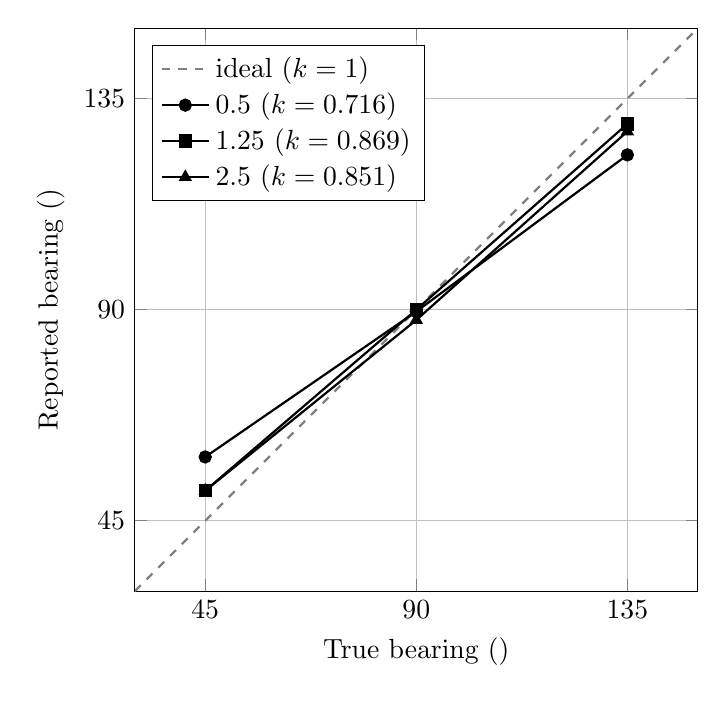
\begin{tikzpicture}
    \begin{axis}[
      width=0.72\textwidth, height=0.72\textwidth,
      xlabel={True bearing (\si{\degree})},
      ylabel={Reported bearing (\si{\degree})},
      xmin=30, xmax=150, ymin=30, ymax=150,
      xtick={45,90,135}, ytick={45,90,135},
      grid=major, legend pos=north west, legend cell align=left,
    ]
      \addplot[dashed, gray, thick, domain=30:150, samples=2] {x};
      \addlegendentry{ideal ($k=1$)}
      \addplot[mark=*, thick] coordinates {(45,58.6) (90,89.6) (135,123.0)};
      \addlegendentry{\SI{0.5}{\metre} ($k=0.716$)}
      \addplot[mark=square*, thick] coordinates {(45,51.4) (90,90.0) (135,129.6)};
      \addlegendentry{\SI{1.25}{\metre} ($k=0.869$)}
      \addplot[mark=triangle*, thick] coordinates {(45,51.4) (90,87.8) (135,128.0)};
      \addlegendentry{\SI{2.5}{\metre} ($k=0.851$)}
    \end{axis}
  \end{tikzpicture}
  \caption{Reported against true bearing in the quiet conditions. All three
  response lines fall inside the ideal diagonal, indicating compression
  towards the frontal axis. The deviation is largest at \SI{0.5}{\metre}.}
  \label{fig:compression}
\end{figure}

The compression is symmetric about the frontal axis: absolute error at
\SI{45}{\degree} and \SI{135}{\degree} does not differ
($H(1) = 0.056$, $p = 0.813$, $\varepsilon^2 = -0.018$, $N = 54$), confirming
that it is a function of off-axis magnitude rather than of rotational
direction.

\subsection{Effect of distance}

The fitted gain differs markedly between \SI{0.5}{\metre} ($k = 0.716$) and the
two larger distances ($k = 0.869$ and $k = 0.851$), which are close to one
another. A Kruskal--Wallis test on absolute error confirms this from an
independent direction. Restricted to off-axis trials, distance has a large
effect ($H(2) = 25.49$, $p < 0.0001$, $\varepsilon^2 = 0.461$, $N = 54$), and
Bonferroni-corrected pairwise comparisons show \SI{0.5}{\metre} differing from
both \SI{1.25}{\metre} ($p_{\text{adj}} = 0.0001$) and \SI{2.5}{\metre}
($p_{\text{adj}} < 0.0001$), while \SI{1.25}{\metre} and \SI{2.5}{\metre} are
indistinguishable ($p_{\text{adj}} = 1.0$).

The two analyses therefore agree on a two-regime response: a near-field regime
below approximately \SI{1}{\metre} in which compression is pronounced, and a
far-field regime beyond it in which the gain is stable at approximately
$k \approx 0.86$. This is consistent with the plane-wave assumption underlying
the array's beamforming being violated at close range.

Restricting the analysis to off-axis trials is necessary rather than
convenient. At \SI{90}{\degree} the model in Equation~\ref{eq:compression}
predicts zero error by construction, so the 29 trials at that bearing
contribute structural zeros that dilute any test of distance or noise. Across
all bearings the same distance comparison is markedly weaker
($H(2) = 8.38$, $p = 0.015$, $\varepsilon^2 = 0.080$).

\subsection{Effect of noise on accuracy}

Background babble degraded orientation accuracy off-axis, raising the median
absolute error from \SI{7.0}{\degree} to \SI{13.0}{\degree}
($H(1) = 18.42$, $p < 0.0001$, $\varepsilon^2 = 0.335$, $N = 54$). The fitted
gain falls correspondingly at every distance (Table~\ref{tab:gain}). As above,
the comparison across all bearings does not reach significance
($p = 0.070$) for the same structural reason.

Figure~\ref{fig:noise} shows the effect as signed error per distance. Under
Equation~\ref{eq:compression} the error is a line through zero at
\SI{90}{\degree} whose slope is $k - 1$, so a steeper line is stronger
compression. Babble steepens the slope at \SI{1.25}{\metre} and
\SI{2.5}{\metre}, increasing the off-axis error by a factor of 1.6 to 2.3. At
\SI{0.5}{\metre}, where compression is already pronounced in quiet, the added
effect appears only at \SI{135}{\degree}.

\begin{figure}[htbp]
  \centering
  \definecolor{quietc}{HTML}{2A78D6}
  \definecolor{babblec}{HTML}{EB6834}
  \begin{tikzpicture}
    \begin{groupplot}[
      group style={group size=3 by 1, horizontal sep=0.4cm,
                   yticklabels at=edge left, ylabels at=edge left},
      scale only axis, width=0.25\textwidth, height=0.25\textwidth,
      xmin=25, xmax=155, ymin=-20, ymax=20,
      xtick={45,90,135}, ytick={-15,-10,-5,0,5,10,15},
      tick label style={font=\footnotesize},
      label style={font=\footnotesize},
      title style={font=\footnotesize},
      grid=major, grid style={line width=0.2pt, draw=black!12},
      axis line style={draw=black!45}, tick style={draw=black!45},
      ylabel={Signed error (\si{\degree})},
      every axis plot/.append style={line width=1pt},
      error bars/error mark=none,
      error bars/error bar style={line width=0.6pt},
    ]
      \nextgroupplot[title={\SI{0.5}{\metre}},
        legend style={at={(0.97,0.97)}, anchor=north east, font=\footnotesize,
                      draw=none, fill=white, cells={anchor=west}}]
      \addplot[black!55, line width=0.6pt, domain=25:155, samples=2, forget plot] {0};
      \addplot[quietc, mark=*, mark size=2.2pt,
               mark options={fill=quietc, draw=white, line width=0.5pt},
               error bars/.cd, y dir=both, y explicit]
        coordinates {(42,13.6) +- (0,1.34) (87,-0.4) +- (0,0.89) (132,-12.0) +- (0,0.71)};
      \addlegendentry{quiet}
      \addplot[babblec, mark=square*, mark size=2.2pt,
               mark options={fill=babblec, draw=white, line width=0.5pt},
               error bars/.cd, y dir=both, y explicit]
        coordinates {(48,13.4) +- (0,0.89) (93,0.4) +- (0,0.55) (138,-15.6) +- (0,0.55)};
      \addlegendentry{babble}

      \nextgroupplot[title={\SI{1.25}{\metre}}, xlabel={True bearing (\si{\degree})}]
      \addplot[black!55, line width=0.6pt, domain=25:155, samples=2, forget plot] {0};
      \addplot[quietc, mark=*, mark size=2.2pt,
               mark options={fill=quietc, draw=white, line width=0.5pt},
               error bars/.cd, y dir=both, y explicit]
        coordinates {(42,6.4) +- (0,1.14) (87,0.0) +- (0,0.0) (132,-5.4) +- (0,0.89)};
      \addplot[babblec, mark=square*, mark size=2.2pt,
               mark options={fill=babblec, draw=white, line width=0.5pt},
               error bars/.cd, y dir=both, y explicit]
        coordinates {(48,12.0) +- (0,1.00) (93,0.0) +- (0,0.0) (138,-12.2) +- (0,2.77)};

      \nextgroupplot[title={\SI{2.5}{\metre}}]
      \addplot[black!55, line width=0.6pt, domain=25:155, samples=2, forget plot] {0};
      \addplot[quietc, mark=*, mark size=2.2pt,
               mark options={fill=quietc, draw=white, line width=0.5pt},
               error bars/.cd, y dir=both, y explicit]
        coordinates {(42,6.4) +- (0,1.52) (87,-2.2) +- (0,1.30) (132,-7.0) +- (0,0.71)};
      \addplot[babblec, mark=square*, mark size=2.2pt,
               mark options={fill=babblec, draw=white, line width=0.5pt},
               error bars/.cd, y dir=both, y explicit]
        coordinates {(48,10.0) +- (0,0.0) (93,-0.5) +- (0,1.00) (138,-12.0) +- (0,1.58)};
      \addplot[only marks, mark=square, mark size=2.2pt,
               mark options={fill=white, draw=babblec, line width=1pt}, forget plot]
        coordinates {(48,10.0)};
      \node[font=\scriptsize, anchor=west] at (axis cs:53,10.0) {$n=1$};
    \end{groupplot}
  \end{tikzpicture}
  \caption{Signed orientation error (reported minus true bearing) in quiet and
  babble, per distance. Points are cell means with $\pm 1$ standard deviation;
  the two conditions are offset horizontally by \SI{3}{\degree} each side of
  the true bearing for legibility. Error at \SI{90}{\degree} is near zero by
  construction, and a steeper slope indicates stronger compression. The open
  marker rests on a single usable trial (four of five missed); the
  \SI{45}{\degree}/\SI{1.25}{\metre} babble mean rests on three trials and the
  \SI{90}{\degree}/\SI{2.5}{\metre} babble mean on four. All other points are
  $n = 5$.}
  \label{fig:noise}
\end{figure}

\subsection{Detection latency}

Latency was measured from the array's first report of voice activity to the
head coming to rest, timed entirely on the device and therefore independent of
operator reaction time. Noise produced the largest single effect observed in
this study, raising the median from \SI{3.413}{\second}
(IQR \SIrange{3.378}{3.667}{\second}) in quiet to \SI{5.170}{\second}
(IQR \SIrange{4.224}{5.534}{\second}) in babble
($H(1) = 48.66$, $p < 0.0001$, $\varepsilon^2 = 0.588$, $N = 83$). Neither
distance ($p = 0.061$) nor bearing ($p = 0.289$) reached significance.

The mechanism is visible in the logs: background noise causes the array's
voice-activity detection to fluctuate, so accumulating five usable bearing
estimates takes substantially longer. A hard lower bound on responsiveness was
also established by direct measurement. Polling the array at \SI{100}{\hertz}
and timing genuine changes in its reported bearing gives an update period of
approximately \SI{128}{\milli\second} (\SI{7.8}{\hertz}). This bounds how
quickly the system can react to a new speaker irrespective of servo speed or
software, and samples taken closer together than this interval return the same
underlying estimate.

\subsection{Detection failures}

The head failed to react in 7 of 90 trials (\SI{7.8}{\percent}). All failures
occurred in the babble condition and were concentrated off-axis: four of five
trials at \SI{45}{\degree}/\SI{2.5}{\metre}, two of five at
\SI{45}{\degree}/\SI{1.25}{\metre}, and one of five at
\SI{90}{\degree}/\SI{2.5}{\metre}. Detection was unaffected in all quiet
conditions and at \SI{135}{\degree} throughout.

The asymmetry between \SI{45}{\degree} and \SI{135}{\degree} under noise is
notable, since orientation accuracy itself is symmetric (Section
\ref{sec:compression}). It is therefore unlikely to originate in the array's
angular response, and more plausibly reflects room geometry or the bearing of
the noise source relative to the two positions, neither of which was
controlled. This is treated as a limitation rather than a finding.

\subsection{Validation of a gain correction}
\label{sec:validation}

Equation~\ref{eq:compression} suggests a direct correction: dividing the
off-axis component of each reading by the fitted $k$ should recover the true
bearing. Since the model was fitted at \SI{45}{\degree}, \SI{90}{\degree} and
\SI{135}{\degree}, it was tested at \SI{60}{\degree}, a bearing not used in the
fit, with the source position verified by protractor.

\begin{table}[htbp]
  \centering
  \caption{Model predictions against observation at \SI{1.25}{\metre}. The
  three fitted bearings agree to within \SI{0.2}{\degree}; the held-out
  bearing is missed by \SI{5.63}{\degree}.}
  \label{tab:validation}
  \begin{tabular}{lcrrr}
    \toprule
    True & In fit & Predicted & Observed & Deviation \\
    \midrule
    \SI{45}{\degree}  & yes & 51.23 & 51.40 & $+0.16$ \\
    \SI{60}{\degree}  & \textbf{no}  & 64.27 & 69.90 & $\mathbf{+5.63}$ \\
    \SI{90}{\degree}  & yes & 90.34 & 90.00 & $-0.34$ \\
    \SI{135}{\degree} & yes & 129.44 & 129.60 & $+0.16$ \\
    \bottomrule
  \end{tabular}
\end{table}

The linear model does not generalise. Applying the correction reduced absolute
error from \SI{8.0}{\degree} to \SI{2.42}{\degree} at the fitted bearing
\SI{45}{\degree}, but only from \SI{9.9}{\degree} to \SI{6.87}{\degree} at the
held-out bearing \SI{60}{\degree}.

The reason is visible in the local gain, $k_{\text{local}} = (\hat{\theta} -
90)/(\theta - 90)$, which is 0.822 at \SI{45}{\degree}, 0.670 at
\SI{60}{\degree} and 0.880 at \SI{135}{\degree}. Absolute error is
\emph{larger} at \SI{60}{\degree} ($+\SI{9.9}{\degree}$, \SI{30}{\degree}
off-axis) than at \SI{45}{\degree} ($+\SI{8.0}{\degree}$, \SI{45}{\degree}
off-axis). A multiplicative gain requires error to grow monotonically with
off-axis angle, which the data contradict. The response is therefore not
describable by a single constant per distance, and the high coefficients of
determination in Table~\ref{tab:gain} reflect only that three near-collinear
points can always be fitted by a line, not that the underlying relationship is
linear.

The compression itself is a robust and reproducible property of the array; it
is the single-constant description of it that is refuted. A correction would
require the angular response to be sampled across the arc and interpolated,
which is left to future work.

\subsection{Limitations}

\begin{itemize}
  \item Head orientation was recorded as the commanded servo angle rather than
  measured per trial. The servo was verified to track its command, so
  mechanical under-rotation is excluded as an explanation for the compression;
  the actuation contribution to total error is nevertheless assumed rather
  than measured.

  \item The apparatus is reproducible to approximately \SI{2}{\degree}. The
  same \SI{45}{\degree} position was reported as \SI{51.4}{\degree} in the main
  experiment and \SI{53.0}{\degree} in the validation session with placement
  confirmed identical, and the in-sample residual after correction was
  $+\SI{2.42}{\degree}$ where zero was expected. No correction validated on
  this apparatus can claim precision beyond this bound.

  \item Cells in the babble condition are thinner because of detection
  failures; \SI{45}{\degree}/\SI{2.5}{\metre} yielded a single usable
  measurement. Miss rate rather than mean error is the appropriate measure for
  that cell. The accuracy effect of noise is also subject to survivorship,
  since it is computed only over trials that produced a bearing at all.

  \item Latency figures are right-censored: they are computed only over trials
  that produced a reading, and the seven failures are precisely the slowest
  cases. The true effect of noise and distance on latency is therefore at
  least as large as reported.

  \item The noise source was not equidistant in bearing from both off-axis
  positions, so the noise factor is partially confounded with bearing (Section
  \ref{sec:validation}).

  \item Gains were fitted from three bearings per distance. The validation in
  Section~\ref{sec:validation} establishes that this is insufficient to
  characterise the response.
\end{itemize}
